\clearpage
\setcounter{page}{1}
\maketitlesupplementary

% Sections of the supplementary material are lettered; \theHsection keeps their hyperref anchors apart from those of the paper.
\setcounter{section}{0}
\renewcommand{\thesection}{\Alph{section}}
\renewcommand{\theHsection}{supp.\Alph{section}}

This supplementary material is organized as follows.
\cref{sec:supp:prelim} gives the protocol and the full results of the preliminary analysis.
\cref{sec:supp:theory} derives the reader metric, the read count, the separable objective, the optimality of the threshold and the error bound of the second pass.
\cref{sec:supp:method} details how \method is calibrated and how it is instantiated on the two models.
\cref{sec:supp:eval} describes the evaluation protocol and the baselines, and \cref{sec:supp:bits} accounts for the precision of every method.
\cref{sec:supp:results,sec:supp:ablation} report additional results and ablations, \cref{sec:supp:cost} the runtime and its cost, \cref{sec:supp:real} the real-world experiments, and \cref{sec:supp:vis} further visualizations.

\section{Preliminary analysis}
\label{sec:supp:prelim}
This section gives the protocol and the full results of the measurements of \cref{sec:observations}.

\paragraph{Setup.}
All measurements use Fast-WAM with 10 denoising steps for the predicted future and 10 for the action, on the first 16 of the 80 calibration contexts with one sampling seed each; the evaluations of \method in \cref{sec:supp:results,sec:supp:ablation} use held-out contexts instead.
The W4A4KV4 model has per-row 4-bit weights fitted by second-order rounding in randomized Hadamard coordinates, per-token symmetric 4-bit activations, and per-head 4-bit cached keys and values.
Every error is measured against the BF16 model on the same observation, instruction and sampling noise.
The action error $A$ is the mean squared error over the first 10 actions of the chunk and the six motor dimensions, and the future error $Z$ is taken over the predicted frames.
The action pathway is protected by giving the activations of the action tokens a second 4-bit pass on the residual of the first, which lowers their rounding error by more than an order of magnitude.

\paragraph{Future swap.}
The future share $\rho$ of \cref{eq:share} is measured by a swap.
After the last denoising step of the video, the future predicted by the quantized model is replaced by the future that the BF16 model predicts for the same context and sampling noise.
The quantized reader, \ie the pass that writes the video cache and the 10 denoising steps of the action, then runs unchanged.
\cref{tab:supp:swap} lists the three models.
Protecting the action pathway removes 16\% of the action error and leaves the future error unchanged.
Restoring the future removes 71.2\% of the remaining action error (95\% bootstrap interval over contexts: 62.1--78.8\%), and the action error falls on every context.
Without the protection of the action pathway, the same swap removes 58.8\% of the action error.

\begin{table}[t]
  \centering
  \small
  \setlength{\tabcolsep}{5pt}
  \begin{tabular}{@{}lcc@{}}
    \toprule
    Model & $A$ ($\times 10^{-4}$) $\downarrow$ & $Z$ $\downarrow$ \\
    \midrule
    W4A4KV4                           & 3.53 & 0.0188 \\
    \quad + protected action pathway  & 2.96 & 0.0188 \\
    \quad + full-precision future     & 0.85 & 0 \\
    \bottomrule
  \end{tabular}
  \caption{Future swap on Fast-WAM. In the last row the quantized reader reads the future predicted by the BF16 model.}
  \label{tab:supp:swap}
\end{table}

\paragraph{Error injection.}
To isolate the effect of the number of reads, the weights are kept in BF16 and an error is injected into one source at a time.
The injected error is the 4-bit rounding error of that source multiplied by random signs, so that it has the energy of the rounding error.
The signs are either drawn once and kept over the denoising steps (frozen) or drawn again at every read (redrawn).
The damage is the future error weighted by the reader metric, $Z_{\bM}$ (\cref{eq:metric-form}).
\cref{tab:supp:reads} reports the two cases and their ratio for three sources.

\begin{table}[t]
  \centering
  \small
  \setlength{\tabcolsep}{5pt}
  \begin{tabular}{@{}lccc@{}}
    \toprule
    Source & Frozen & Redrawn & Ratio \\
    \midrule
    Observation tokens          & 11.56 & 3.68 & 3.1$\times$ \\
    Cache of the observed frame & 3.29  & 1.49 & 2.2$\times$ \\
    Cache of the text           & 0.48  & 0.23 & 2.1$\times$ \\
    \bottomrule
  \end{tabular}
  \caption{Reader-weighted future error $Z_{\bM}$ ($\times 10^{-3}$) caused by an injected error of fixed energy whose realization is kept over the denoising steps (frozen) or redrawn at every read.}
  \label{tab:supp:reads}
\end{table}

\paragraph{Accumulation over the denoising steps.}
A policy call has 21 phases: the 10 denoising steps of the video, the pass that writes the video cache, and the 10 denoising steps of the action.
We run one phase at W4A4KV4 and all others in BF16, and compare the sum of the errors of the 10 video steps taken one at a time with the error when the 10 steps are quantized together (\cref{tab:supp:steps}).
Together, the 10 steps cause 2.50$\times$ the reader-weighted future error of the sum, and 1.54$\times$ its action error.
The first three denoising steps carry 70\% of the sum.

\begin{table}[t]
  \centering
  \small
  \setlength{\tabcolsep}{5pt}
  \begin{tabular}{@{}lcc@{}}
    \toprule
    Quantized video steps & $Z_{\bM}$ ($\times 10^{-3}$) & $A$ ($\times 10^{-4}$) \\
    \midrule
    Step 1 alone  & 4.79 & 0.38 \\
    Step 2 alone  & 3.59 & 0.52 \\
    Step 3 alone  & 1.46 & 0.11 \\
    Step 4 alone  & 0.75 & 0.06 \\
    Step 5 alone  & 0.66 & 0.05 \\
    Step 6 alone  & 0.23 & 0.03 \\
    Step 7 alone  & 0.31 & 0.03 \\
    Step 8 alone  & 0.36 & 0.03 \\
    Step 9 alone  & 0.49 & 0.03 \\
    Step 10 alone & 1.37 & 0.03 \\
    \midrule
    Sum of the 10 steps & 14.0 & 1.27 \\
    All 10 steps        & 35.0 & 1.95 \\
    \bottomrule
  \end{tabular}
  \caption{Errors on Fast-WAM when only some of the video denoising steps run at W4A4KV4 and every other phase runs in BF16.}
  \label{tab:supp:steps}
\end{table}

\paragraph{Reader metric.}
The effective rank of $\bM$ is $\tr(\bM)^2 / \tr(\bM^2)$.
The stability of the locations is the correlation between the diagonals of $\bM$ estimated on two disjoint halves of the calibration contexts (0.86); on the tokens of the first predicted frame, the maps of the two halves correlate at 0.84.
The overlap between two eigenspaces is $\|\mathbf{E}_1^\top \mathbf{E}_2\|_F^2 / r$, where $\mathbf{E}_1$ and $\mathbf{E}_2$ hold the $r = 32$ leading eigenvectors estimated on the two halves; it is 1 for identical subspaces.
The frame shown in \cref{fig:obs:gaze} is the fourth decoded frame of the BF16 prediction for one context of the Goal suite.


\section{Derivations}
\label{sec:supp:theory}
This section derives the statements of \cref{sec:method} in the order in which they appear there.
Throughout, $\Delta\bz = \hat\bz - \bz^\star$ is the error of the predicted future, a rounding error is modeled as zero-mean noise that is uncorrelated across sources, and expansions are taken around the full-precision model.

\subsection{Reader metric and reader error}
\label{sec:supp:theory:metric-kl}
\paragraph{The reader metric is the Hessian of the reader error.}
For a context $c$, write the reader error of \cref{eq:reader-kl} as a function of the future, $K_c(\bz) = k\big(R(\bo_c, \ell_c, \bz)\big)$ with $k(\ba) = \mathrm{KL}\big(\pi(\ba^\star_c)\,\|\,\pi(\ba)\big)$.
A KL divergence is non-negative and vanishes when its two arguments coincide, so $k$ has a minimum at $\ba^\star_c$: $k(\ba^\star_c) = 0$ and $\nabla k(\ba^\star_c) = \mathbf{0}$.
The chain rule gives
\begin{equation}
  \nabla^2_{\bz} K_c = \bJ_c^\top\, \nabla^2 k\; \bJ_c + \sum_i \frac{\partial k}{\partial a_i}\, \nabla^2_{\bz} R_i ,
  \label{eq:supp:chain}
\end{equation}
and the second term vanishes at $\bz^\star_c$ because $\nabla k(\ba^\star_c) = \mathbf{0}$.
The Gauss--Newton matrix is therefore the exact Hessian at the full-precision future, not an approximation of it.
Since $\pi$ maps every action coordinate to its own histogram, $k$ is a sum over coordinates and $\nabla^2 k(\ba^\star_c)$ is the diagonal matrix $\bD_c$ of \cref{sec:method:metric}; its $i$-th entry is the Fisher information of the histogram of coordinate $i$ with respect to that coordinate.
Hence
\begin{equation}
  K_c(\bz^\star_c + \Delta\bz) = \tfrac12\, \Delta\bz^\top \bJ_c^\top \bD_c\, \bJ_c\, \Delta\bz + O\big(\|\Delta\bz\|^3\big).
  \label{eq:supp:k2}
\end{equation}

\paragraph{One metric for every error outside the reader.}
Consider a rounding error that enters outside the reader, at any layer, token or denoising step of the computation that writes the future.
The reader itself is unchanged, so the action it produces differs from the full-precision action only because its input differs, by $\Delta\bz$.
By \cref{eq:supp:k2}, the damage of such an error is a quadratic form of $\Delta\bz$ in the matrix $\bJ_c^\top \bD_c \bJ_c$, whatever its origin.
Averaging over contexts, each normalized to unit trace, and replacing the per-context matrix by the average $\bM$ of \cref{eq:metric} gives the reader-weighted future error $Z_{\bM}$.
This replacement is what makes the metric reusable: \cref{sec:supp:prelim} shows that the diagonal of $\bM$ is stable across contexts.

\paragraph{Relation between the terms of the objective.}
With the form of \cref{eq:metric-form}, the reader-weighted future error splits as
\begin{equation}
  Z_{\bM} = (1-\alpha)\,\frac{d}{\tr\bM_r}\, Z_{\bM_r} + \alpha\, Z ,
  \label{eq:supp:split}
\end{equation}
and by \cref{eq:supp:k2} the first term is, up to the truncation to $\bM_r$ and the normalization of each context, proportional to the reader error $K$.
To second order, $\lambda_{\bM} Z_{\bM} + \beta K$ is thus a combination of the reader error $K$ and the uniform future error $Z$ with weights set by $\lambda_{\bM}$, $\beta$ and $\alpha$.
The two terms differ beyond second order, where $K$ also captures the saturation of the histogram $\pi$.

\subsection{Read count}
\label{sec:supp:theory:count}
Let $u$ be a source whose rounding error $\be_{u,s}$ enters at denoising step $s = 1, \dots, T$, with $\mathbb{E}[\be_{u,s}] = \mathbf{0}$ and $\mathbb{E}[\be_{u,s}\be_{u,s}^\top] = \sigma_u^2\, \mathbf{I}$, independent of the Jacobians $\bJ_{u,s}$.
To first order $\Delta\bz = \sum_s \bJ_{u,s}\,\be_{u,s}$, so the expected damage in the reader metric is
\begin{equation}
  \mathbb{E}\big[\Delta\bz^\top \bM\, \Delta\bz\big] = \sum_{s, s'} \mathbb{E}\big[\be_{u,s}^\top\, \bJ_{u,s}^\top\, \bM\, \bJ_{u,s'}\, \be_{u,s'}\big].
  \label{eq:supp:damage}
\end{equation}

\paragraph{Fresh and frozen errors.}
For a fresh error, the realizations of different steps are uncorrelated, $\mathbb{E}[\be_{u,s}\be_{u,s'}^\top] = \sigma_u^2\, \delta_{ss'}\, \mathbf{I}$, and only the terms with $s = s'$ remain:
\begin{equation}
  \mathbb{E}\big[\Delta\bz^\top \bM\, \Delta\bz\big] = \sigma_u^2 \sum_s \bOmega_u(s, s) = \sigma_u^2\, \tr\bOmega_u .
\end{equation}
For a frozen error, $\be_{u,s} = \be_u$ at every step, so $\mathbb{E}[\be_{u,s}\be_{u,s'}^\top] = \sigma_u^2\, \mathbf{I}$ for every pair of steps and
\begin{equation}
  \mathbb{E}\big[\Delta\bz^\top \bM\, \Delta\bz\big] = \sigma_u^2 \sum_{s,s'} \bOmega_u(s, s') = \sigma_u^2\, \bone^\top \bOmega_u\, \bone ,
\end{equation}
with $\bOmega_u$ as in \cref{eq:kernel}.
The read count $n_u$ of \cref{eq:count} is the ratio of the two.

\paragraph{Bounds.}
$\bOmega_u$ is symmetric because $\bM$ is, and it is positive semidefinite: for any $\mathbf{v} \in \mathbb{R}^T$,
\begin{equation}
  \mathbf{v}^\top \bOmega_u\, \mathbf{v} = \mathbb{E}\,\Big\| \bM^{1/2} \sum_s v_s\, \bJ_{u,s} \Big\|_F^2 \;\ge\; 0 .
\end{equation}
Its largest eigenvalue is therefore at most its trace, and
\begin{equation}
  0 \;\le\; \bone^\top \bOmega_u\, \bone \;\le\; \lambda_{\max}(\bOmega_u)\, \|\bone\|^2 \;\le\; T\, \tr\bOmega_u ,
\end{equation}
which gives $n_u \in [0, T]$.
The upper bound is attained when $\bM^{1/2}\bJ_{u,s}$ is the same at every step, \ie when the effects of the $T$ reads add coherently; $n_u = 1$ when the effects of different steps are orthogonal in the reader metric, which is the case that a per-step sensitivity assumes; and $n_u < 1$ when they partly cancel.

\paragraph{Measurement by intervention.}
Multiplying a rounding error by random signs keeps the magnitude of each of its entries, hence its energy, and makes it zero-mean.
Keeping one sign pattern over the denoising steps realizes the frozen case and redrawing it at every read the fresh case, so the ratio of the two measured $Z_{\bM}$ estimates $n_u$ without differentiating through the sampler, and at the error level of the 4-bit quantizer rather than to first order.

\subsection{Separable objective}
\label{sec:supp:theory:separable}
Stack the rounding errors of all sources into one vector $\be$.
Each term of \cref{eq:objective} is non-negative and vanishes at $\be = \mathbf{0}$, so $\mathcal{L}$ has no first-order term:
\begin{equation}
  \mathcal{L}(\be) = \tfrac12\, \be^\top \mathbf{G}\, \be + O\big(\|\be\|^3\big), \qquad \mathbf{G} = \nabla^2_{\be}\, \mathcal{L}\,\big|_{\be = \mathbf{0}} \succeq 0 .
\end{equation}
Since the errors of different sources are uncorrelated and zero-mean, the expectation of every cross term between two sources vanishes, and the expected objective is a sum over sources,
\begin{equation}
  \mathbb{E}\big[\mathcal{L}\big] \approx \tfrac12 \sum_u \mathbb{E}\big[\be_u^\top\, \mathbf{G}_{uu}\, \be_u\big],
  \label{eq:supp:sum}
\end{equation}
where $\mathbf{G}_{uu}$ is the block of $\mathbf{G}$ that belongs to source $u$ over all the steps at which it is read.

\paragraph{Activations and caches.}
For a unit $u$ with error variance $\sigma_u^2$, the computation of \cref{sec:supp:theory:count}, with the curvature of $\mathcal{L}$ in place of $\bM$, gives $\sigma_u^2\, \tr\bOmega_u$ for a fresh error and $n_u$ times as much for a frozen one.
With $\omega_u = \tr\bOmega_u$, the term of unit $u$ is $n_u\, \omega_u\, \sigma_u^2$, where $n_u = 1$ for fresh sources.
Refinement changes only $\sigma_u^2$, which gives the sum of \cref{eq:separable}.

\paragraph{Weights.}
The weights are rounded to 4 bits before any unit is refined, and refinement does not change their errors.
Their blocks of $\mathbf{G}$ therefore add the same amount to $\mathcal{L}$ for every choice of $r$, the constant $C_{\bW}$ of \cref{eq:separable}.

\subsection{Optimality of the threshold}
\label{sec:supp:theory:threshold}
Let $b_u = n_u\, \omega_u\, \big(\sigma_u^2(0) - \sigma_u^2(1)\big) \ge 0$ be the damage that refining unit $u$ removes, and $c_u > 0$ its cost.
Minimizing the sum of \cref{eq:separable} under the budget is the 0/1 knapsack problem
\begin{equation}
  \max_{r \in \{0,1\}^N}\; \sum_u b_u\, r_u \quad \text{s.t.} \quad \sum_u c_u\, r_u \le B .
  \label{eq:supp:knapsack}
\end{equation}
Since refinement divides $\sigma_u^2$ by at least 196 (\cref{sec:supp:theory:refine}), $b_u$ lies between $\tfrac{195}{196}$ and $1$ times $n_u\, \omega_u\, \sigma_u^2(0)$, so ranking the units by $b_u / c_u$ and by the ratio of \cref{eq:threshold} differ by less than 0.6\%.

\paragraph{Proposition.}
For any $\mu \ge 0$, let $r^\mu_u = 1$ if $b_u / c_u \ge \mu$ and $r^\mu_u = 0$ otherwise, and let $B(\mu) = \sum_u c_u\, r^\mu_u$ be the budget it spends.
Then $r^\mu$ solves \cref{eq:supp:knapsack} for $B = B(\mu)$.

\paragraph{Proof.}
By construction, $r^\mu$ maximizes $(b_u - \mu\, c_u)\, r_u$ for every unit separately, hence it maximizes $\sum_u (b_u - \mu\, c_u)\, r_u$ over $\{0,1\}^N$.
For any $r$ with $\sum_u c_u\, r_u \le B(\mu)$,
\begin{align}
  \sum_u b_u\, r_u
    &= \sum_u (b_u - \mu\, c_u)\, r_u + \mu \sum_u c_u\, r_u \nonumber\\
    &\le \sum_u (b_u - \mu\, c_u)\, r^\mu_u + \mu\, B(\mu) = \sum_u b_u\, r^\mu_u ,
\end{align}
which proves the claim.
This is the generalized Lagrange multiplier argument of Everett.

\paragraph{General budgets.}
For a budget $B$ that no threshold spends exactly, sort the units by decreasing $b_u / c_u$ and refine them in this order until the next unit no longer fits.
Filling the remaining budget with a fraction of that unit solves the continuous relaxation of \cref{eq:supp:knapsack}, whose value bounds that of the 0/1 problem from above.
The threshold solution therefore removes at least the optimal damage minus the damage removed by one unit, $\max_u b_u$.
A unit is one token at one denoising step or one cached token, among more than $10^3$ refined units per policy call, so this gap is negligible.

\subsection{Error bound of the second pass}
\label{sec:supp:theory:refine}
Let $\bx$ be the activation of a token, quantized without clipping with the scale $\varsigma_1 = \max|\bx| / 7$ of \cref{sec:prelim}.
Every entry of $\bx / \varsigma_1$ lies in $[-7, 7]$, so $\mathbf{q}_1$ is a 4-bit integer vector and the residual $\mathbf{r}_1 = \bx - \varsigma_1 \mathbf{q}_1$ satisfies $|r_{1,i}| \le \varsigma_1 / 2$.
The second pass quantizes $\mathbf{r}_1$ in the same way with $\varsigma_2 = \max|\mathbf{r}_1| / 7 \le \varsigma_1 / 14$, so $\mathbf{q}_2$ is again a 4-bit integer vector and
\begin{equation}
  \big|x_i - \hat x_i\big| = \big|r_{1,i} - \varsigma_2\, q_{2,i}\big| \;\le\; \frac{\varsigma_2}{2} \;\le\; \frac{\varsigma_1}{28} .
\end{equation}
The worst-case error is 14 times smaller than that of one pass.
Under the standard model of a rounding error that is uniform within one step of the grid, its power is $\varsigma^2 / 12$, so the second pass lowers it from $\varsigma_1^2 / 12$ to $\varsigma_2^2 / 12 \le \varsigma_1^2 / (196 \cdot 12)$, a factor of at least 196.
The step of the refined grid, $\varsigma_2 \le \max|\bx| / 98$, lies between those of a 7-bit grid ($\max|\bx| / 63$) and an 8-bit grid ($\max|\bx| / 127$).
Because the layer is linear, $\bW \hat\bx = \varsigma_1\, \bW \mathbf{q}_1 + \varsigma_2\, \bW \mathbf{q}_2$: the refined token is served by two products with 4-bit operands, and no operand wider than 4 bits enters a matrix product.

\section{Method details}
\label{sec:supp:method}
\cref{alg:laq} summarizes \method.
This section gives the settings behind each of its steps; \cref{tab:supp:hparams} collects the hyperparameters.

\begin{algorithm}[H]
  \caption{\method}
  \label{alg:laq}
  \small
  \begin{algorithmic}[1]
    \Require full-precision WAM $\bW$, calibration contexts $\mathcal{C}$, budget $B$
    \Statex \textbf{Offline}
    \State Estimate the reader metric $\bM$ from reader probes on $\mathcal{C}$ \Comment{\cref{sec:method:metric}}
    \State Measure the read counts $n_u$ and the step profile $\phi_s$ by error injection \Comment{\cref{sec:method:count}}
    \State Round every $\bW_l$ to 4 bits by second-order rounding; set the threshold $\mu$ from $B$ \Comment{\cref{sec:method:alloc}}
    \Statex \textbf{At every control step}
    \State Select the tokens that satisfy \cref{eq:threshold} under the current gaze
    \State Run the 4-bit model; give the selected tokens a second 4-bit pass in the denoising loop and in the cache \Comment{\cref{sec:method:refine}}
    \State Update the gaze from the attention of the action tokens
  \end{algorithmic}
\end{algorithm}

\paragraph{Reader error.}
The soft histogram $\pi$ of \cref{eq:reader-kl} standardizes each of the six motor coordinates of the first 10 actions by its mean and standard deviation over the BF16 actions on the 80 calibration contexts, with the standard deviation floored at 0.02.
It then assigns the coordinate to 16 bins, whose 15 interior edges are evenly spaced in $[-3.5, 3.5]$, under Gaussian noise of standard deviation 0.375.
$K$ is the mean over these 60 coordinates of the KL divergence between the bin probabilities of the BF16 action and those of the action read from the quantized future.

\paragraph{Estimating the reader metric.}
The metric is estimated on the BF16 model alone, on the 80 calibration contexts with four Rademacher probes each.
For every context, the BF16 model first predicts the future $\bz^\star_c$; the reader then runs from this future with the sampling noise of the context, and one reverse pass through the reader per probe gives $\mathbf{v} = \bJ_c^\top(\bD_c^{1/2}\boldsymbol{\epsilon})$.
Forming $\bJ_c$ itself would take one reverse pass per action coordinate and a dense matrix over the latent.
Only the predicted frames enter the metric, since the observed frame is fixed by the input.
The estimate of a context is the mean of $\mathbf{v}\mathbf{v}^\top$ over its probes, normalized to unit trace so that no single context dominates, and $\bM$ is the mean over contexts.
We never form the $d \times d$ matrix: the 320 normalized probes are stacked into a $320 \times d$ matrix, whose thin singular value decomposition gives the eigendirections and whose squared columns give the diagonal.
$\bM_r$ keeps the $r = 32$ leading eigendirections, which carry 52\% of the trace, and the diagonal of the remainder, and \cref{eq:metric-form} mixes in the identity with $\alpha = 0.1$.
The estimation takes one forward pass of the model and four reverse passes of the reader per context.

\paragraph{Weights of the objective.}
The terms of \cref{eq:objective} have different scales, so we weight them once, on the model without refinement: $\lambda_{\bM}$ is the ratio between the mean action error $A$ and the mean reader-weighted future error $Z_{\bM}$ over the calibration contexts, which makes the two terms contribute equally before any token is refined.
This gives $\lambda_{\bM} = 0.0101$ on Fast-WAM and $\lambda_{\bM} = 3.11$ on Cosmos-Policy.
By \cref{sec:supp:theory:metric-kl}, the reader error $K$ agrees with the low-rank part of $Z_{\bM}$ to second order, so during calibration its weight is carried by $\lambda_{\bM}$; $K$ itself is the error we report.

\paragraph{Units, classes and costs.}
A unit is one token whose activations are rounded in one pass of the model, or one token whose keys and values are cached.
Refining an activation unit adds one row to every 4-bit matrix product that reads the token in that pass, and refining a cached unit stores a second 4-bit code for each of its keys and values.
Both costs are counted in the same unit, the number of additional 4-bit operands, and the budget $B$ is 15\% of the 4-bit operands of the activations and caches of one policy call.
Units are grouped into classes that share a read count: on Fast-WAM, the text tokens, the tokens of the observed frame, the cache of the observed frame, the cache of the predicted future, and the future tokens of each of the 10 denoising steps and of the pass that writes the cache.
The activations of the action tokens are always refined; they are 5.9\% of the activation operands on Fast-WAM.

\paragraph{Read counts and step profile.}
The read counts of the frozen classes are those of \cref{tab:supp:reads}: 3.1 for the tokens of the observed frame, 2.2 for its cache and 2.1 for the text cache.
The cache of the predicted future and the text cache of the action expert are written after the future is complete, so they do not change $Z_{\bM}$; measured on the action error, their read counts are 1.1 and 1.2.
The damage of a class is the decrease of the objective when the whole class is refined and nothing else changes, measured on 16 calibration contexts with the quantized model; for the future tokens, the damages of the 11 passes form the step profile $\phi_s$.
A class whose refinement does not lower the objective receives no budget.
On Fast-WAM, the tokens of the observed frame account for 34\% of the objective, and the first three denoising steps for 7.5\%, 11.9\% and 13.3\%; no later step exceeds 6\%.
The damage of a class is divided among its tokens in proportion to the gaze, and the threshold of \cref{eq:threshold} then fixes how many tokens of each class are refined (\cref{tab:supp:alloc}).
At run time these numbers stay fixed and the gaze decides which tokens they are.

\paragraph{Gaze at run time.}
For Fast-WAM, the gaze of a future token is the attention mass that the action tokens place on its cached keys, summed over the layers, the heads and the 10 denoising steps of the action.
The gaze of an observation token adds the mass that the action tokens place on it directly to the mass propagated through the future tokens, $\sum_j g_j\, a_{j \to i}$, where $a_{j \to i}$ is taken from the pass that writes the cache.
The gaze of one policy call selects the tokens of the next, and the first call of an episode uses the offline gaze.
This relies on the gaze changing slowly along an episode.
Over the LIBERO-Plus episodes, the sets of future tokens selected at two consecutive policy calls have a Jaccard overlap of 0.70, whereas the set selected by the offline gaze overlaps with them by 0.21: the tokens that the reader depends on move with the scene, and the previous call tracks them.

\paragraph{Instantiation on Cosmos-Policy.}
Cosmos-Policy denoises nine latent slots of 196 tokens jointly in one transformer: four conditioning slots that hold the observation, the action, two future images, and two auxiliary slots that hold the future proprioception and the value.
One policy call evaluates the denoiser five times.
Three points differ from Fast-WAM.
(i) The reader starts from the state of the solver before the last evaluation, and the reader metric is defined on the future-image slots of this state.
(ii) Only the text tokens are written once and read at every evaluation; the observation tokens are recomputed at every evaluation, so every other class is fresh.
The classes are the token groups (observation, future, auxiliary, action), separately for activations and for keys and values, at each of the five evaluations.
(iii) The gaze is the self-attention mass that the action tokens place on each token within one evaluation; the gaze of one evaluation selects the tokens of the next, the first evaluation of a call uses the last gaze of the previous call, and the first call of an episode uses the offline gaze.
Between consecutive evaluations, the quarter of the future tokens with the largest gaze overlaps by 0.99.
The rounding of the weights, the refinement, the budget and the objective are those of Fast-WAM.

\begin{table}[t]
  \centering
  \small
  \setlength{\tabcolsep}{4pt}
  \begin{tabular}{@{}ll@{}}
    \toprule
    Setting & Value \\
    \midrule
    \multicolumn{2}{@{}l}{\emph{Quantizers}} \\
    \hspace{0.5em}Weights & 4 bits, scale per output row \\
    \hspace{0.5em}Weight rounding & GPTQ, Hadamard coordinates \\
    \hspace{0.5em}Activations & 4 bits, scale per token \\
    \hspace{0.5em}Keys and values & 4 bits, scale per token and head \\
    \hspace{0.5em}Second pass & 4 bits on the residual \\
    \midrule
    \multicolumn{2}{@{}l}{\emph{Reader metric}} \\
    \hspace{0.5em}Contexts, probes per context & 80, 4 \\
    \hspace{0.5em}Rank $r$, identity weight $\alpha$ & 32, 0.1 \\
    \hspace{0.5em}Histogram $\pi$ & 16 bins, noise 0.375 \\
    \midrule
    \multicolumn{2}{@{}l}{\emph{Allocation}} \\
    \hspace{0.5em}Contexts & 16 \\
    \hspace{0.5em}Budget $B$ & 15\% of the operands \\
    \hspace{0.5em}$\lambda_{\bM}$ & mean $A$ / mean $Z_{\bM}$ \\
    \hspace{0.5em}Gaze of the first policy call & offline \\
    \bottomrule
  \end{tabular}
  \caption{Hyperparameters of \method, shared by Fast-WAM and Cosmos-Policy.}
  \label{tab:supp:hparams}
\end{table}

\section{Evaluation details}
\label{sec:supp:eval}
\paragraph{Calibration and evaluation.}
Fast-WAM denoises the future latent in 10 steps and a 32-step action chunk in 10 steps, and the robot executes the first 10 actions before replanning.
Cosmos-Policy runs its official sampler with 5 denoising steps, and the robot executes the full 16-step action chunk.
Calibration uses 80 observations from the original LIBERO suites, 20 from each suite, shared by all methods that calibrate.
On LIBERO-Plus, every method runs the same 840 variants, 30 for each suite and perturbation dimension.
On LIBERO, every method runs the 40 tasks from 21 official initial states each, 840 episodes in total.
Initial states, environment seeds and sampling noise are matched across methods, so that episodes are paired, and success rates are averaged over episodes.
An episode ends on success or after 400 control steps (700 on the Long suite).

\paragraph{Baselines.}
All baselines quantize the linear layers of the transformer blocks to W4A4 and keep the cached keys and values in BF16.
QuaRot and SpinQuant rotate the input of every linear layer by block rotations of size 128 and fold them into its weights.
QuaRot uses fixed randomized Hadamard blocks; SpinQuant,
ViDiT-Q and SVDQuant calibrate on the same 80 contexts as \method.
ViDiT-Q follows the linear layer of its official code: a channel-balancing mask with exponent 0.5665, a randomized Hadamard rotation, two-stage weight quantization with one scale per group of 128, and asymmetric per-token 4-bit activations; on Cosmos-Policy, nine linear layers take 8-bit weights within the same average budget.
SVDQuant follows DeepCompressor: a per-layer search of the smoothing exponents, a rank-32 BF16 branch fitted iteratively to the weight residual, 4-bit weights and dynamic 4-bit activations with one scale per group of 64, and unsigned activations at the input of the second feed-forward layer.

\section{Precision accounting}
\label{sec:supp:bits}
This section explains the average bits of \cref{tab:main}.

\paragraph{Weights.}
The average covers the quantized linear layers and counts every stored quantity: the codes, the scales and any component kept at higher precision.
\method stores 4-bit codes and one 32-bit scale per output row, 4.01 bits per weight, and nothing else.
ViDiT-Q adds the zero points of its groups and its channel-balancing vectors, and on Cosmos-Policy the nine layers that take 8-bit weights; its averages are 4.33 bits on Fast-WAM and 4.29 bits on Cosmos-Policy.
SVDQuant uses groups of 64 and keeps a 16-bit branch of rank 32 next to every layer, which gives 4.81 and 4.89 bits.
For all methods, the interface layers (0.01\% of the weights) stay in BF16, and the timestep-conditioning layers, whose inputs depend only on the denoising step, are stored as exact per-step tables; neither enters the average.

\paragraph{Activations and caches.}
The baselines quantize every activation once at 4 bits and keep the cached keys and values in BF16.
For \method, a refined unit holds two 4-bit codes, so the average is 4 bits times one plus the share of refined operands.
The share is taken over the operands of one policy call, where an activation counts once for every matrix product that reads it and a cached entry counts once.
\cref{tab:supp:bits} gives this share for each class, and \cref{tab:supp:alloc} the number of refined tokens behind it.
On Fast-WAM, the refined activations split almost evenly between the action tokens, the tokens of the observed frame and the future tokens, and only 33 of the 196 future tokens keep a second code in the cache.
On Cosmos-Policy, most of the refined activations are those of the action tokens, and the cache takes a larger share: the keys and values of the action tokens are refined at four of the five evaluations.

\begin{table}[t]
  \centering
  \small
  \setlength{\tabcolsep}{5pt}
  \begin{tabular}{@{}lcc@{}}
    \toprule
    Refined operands (\%) & Fast-WAM & Cosmos-Policy \\
    \midrule
    \multicolumn{3}{@{}l}{\emph{Activations}} \\
    \hspace{0.5em}Action tokens       & 5.9  & 11.1 \\
    \hspace{0.5em}Observation tokens  & 4.1  & 0.0 \\
    \hspace{0.5em}Future tokens       & 5.4  & 0.6 \\
    \hspace{0.5em}Auxiliary tokens    & --   & 2.7 \\
    \hspace{0.5em}Total               & 15.4 & 14.4 \\
    \hspace{0.5em}Average bits        & 4.62 & 4.58 \\
    \midrule
    \multicolumn{3}{@{}l}{\emph{Cached keys and values}} \\
    \hspace{0.5em}Total               & 6.0  & 17.6 \\
    \hspace{0.5em}Average bits        & 4.24 & 4.70 \\
    \bottomrule
  \end{tabular}
  \caption{Share of the 4-bit operands of one policy call that \method refines, by class, and the resulting average bits.}
  \label{tab:supp:bits}
\end{table}

\begin{table}[t]
  \centering
  \small
  \setlength{\tabcolsep}{2.6pt}
  \begin{tabular}{@{}lccccccccccc@{}}
    \toprule
    \multicolumn{12}{@{}l}{\emph{Fast-WAM: future tokens refined at each pass (of 196)}} \\
    Pass    & 1 & 2 & 3 & 4 & 5 & 6 & 7 & 8 & 9 & 10 & W \\
    Tokens  & 23 & 34 & 40 & 0 & 0 & 14 & 0 & 0 & 2 & 0 & 18 \\
    \midrule
    \multicolumn{12}{@{}l}{\emph{Fast-WAM: other classes}} \\
    \multicolumn{8}{@{}l}{Observation tokens (activations)} & \multicolumn{4}{r@{}}{98 of 98} \\
    \multicolumn{8}{@{}l}{Cache of the observed frame}      & \multicolumn{4}{r@{}}{0 of 98} \\
    \multicolumn{8}{@{}l}{Cache of the predicted future}    & \multicolumn{4}{r@{}}{33 of 196} \\
    \multicolumn{8}{@{}l}{Text tokens and their cache}      & \multicolumn{4}{r@{}}{0} \\
    \bottomrule
  \end{tabular}

  \vspace{4pt}
  \setlength{\tabcolsep}{5pt}
  \begin{tabular}{@{}lccccc@{}}
    \toprule
    \multicolumn{6}{@{}l}{\emph{Cosmos-Policy: tokens refined at each evaluation}} \\
    Class & 1 & 2 & 3 & 4 & 5 \\
    \midrule
    Observation, activations (784) & 0   & 0   & 0   & 0  & 1 \\
    Observation, cache (784)       & 206 & 0   & 0   & 0  & 7 \\
    Future, activations (392)      & 0   & 0   & 0   & 19 & 36 \\
    Future, cache (392)            & 0   & 331 & 0   & 24 & 0 \\
    Auxiliary, activations (392)   & 0   & 238 & 0   & 0  & 0 \\
    Auxiliary, cache (392)         & 0   & 0   & 287 & 0  & 0 \\
    Action, cache (196)            & 196 & 196 & 196 & 0  & 196 \\
    \bottomrule
  \end{tabular}
  \caption{Allocation of \method under the 15\% budget.
  For Fast-WAM, passes 1--10 are the denoising steps of the future and W is the pass that writes the cache.
  The activations of the action tokens are always refined and are not listed.
  The number of tokens of each class is given in parentheses.}
  \label{tab:supp:alloc}
\end{table}

\section{Additional results}
\label{sec:supp:results}
\cref{tab:supp:dims} breaks the LIBERO-Plus results of \cref{tab:main} down by perturbation dimension; each entry covers 120 episodes, 30 from each suite.
On Fast-WAM, the baselines lose the most under shifted camera viewpoints (10.9--17.5 points below BF16) and under sensor noise (5.8--10.8 points).
\method loses 2.5 points on each.
On Cosmos-Policy, all methods stay within a few points of BF16 on every dimension, in line with its smaller overall loss.

\paragraph{Fidelity of the predicted future.}
We also measure directly how much of the predicted future \method preserves.
On the 80 held-out queries of \cref{sec:supp:ablation} (40 contexts, two sampling seeds each), we compare the future predicted by \method and by the same 4-bit weights without refinement with the future predicted by the BF16 model under the same sampling noise.
Refinement lowers the future error $Z$ from 0.034 to 0.020, a reduction of 42\%.
On the first seed of every context, whose futures we also decoded, it lowers the error of the first predicted frame, which carries most of the reader metric, from 0.011 to 0.007, and on 16 of these contexts the decoded frames of \method are 1.4\,dB closer to those of BF16 (PSNR of 30.1\,dB against 28.8\,dB).

\begin{table*}[t]
  \centering
  \small
  \setlength{\tabcolsep}{5pt}
  \begin{tabular}{@{}llcccccccc@{}}
    \toprule
    Model & Method & Camera & Robot init. & Language & Lighting & Background & Noise & Layout & Avg. \\
    \midrule
    \multirow{6}{*}{Fast-WAM}
      & BF16      & 61.7 & 73.3 & 93.3 & 90.0 & 70.0 & 65.8 & 89.2 & 77.6 \\
    \cmidrule(l){2-10}
      & QuaRot    & 44.2 & 68.3 & 94.2 & 92.5 & 65.0 & 55.0 & 85.8 & 72.1 \\
      & SpinQuant & 50.8 & 63.3 & 93.3 & 93.3 & 63.3 & 55.0 & 85.0 & 72.0 \\
      & ViDiT-Q   & 44.2 & 70.8 & 95.0 & 88.3 & 66.7 & 60.0 & 84.2 & 72.7 \\
      & SVDQuant  & 46.7 & 68.3 & 94.2 & 91.7 & 65.8 & 56.7 & 87.5 & 73.0 \\
      & \cellcolor{gray!12}\method & \cellcolor{gray!12}59.2 & \cellcolor{gray!12}72.5 & \cellcolor{gray!12}94.2 & \cellcolor{gray!12}90.8 & \cellcolor{gray!12}70.0 & \cellcolor{gray!12}63.3 & \cellcolor{gray!12}85.0 & \cellcolor{gray!12}76.4 \\
    \midrule
    \multirow{6}{*}{Cosmos-Policy}
      & BF16      & 75.0 & 55.8 & 95.0 & 99.2 & 84.2 & 89.2 & 85.8 & 83.5 \\
    \cmidrule(l){2-10}
      & QuaRot    & 75.8 & 51.7 & 91.7 & 99.2 & 80.8 & 87.5 & 86.7 & 81.9 \\
      & SpinQuant & 72.5 & 51.7 & 93.3 & 99.2 & 75.0 & 85.8 & 84.2 & 80.2 \\
      & ViDiT-Q   & 78.3 & 53.3 & 92.5 & 99.2 & 83.3 & 87.5 & 85.8 & 82.9 \\
      & SVDQuant  & 75.8 & 53.3 & 93.3 & 99.2 & 81.7 & 90.8 & 85.8 & 82.9 \\
      & \cellcolor{gray!12}\method & \cellcolor{gray!12}75.8 & \cellcolor{gray!12}53.3 & \cellcolor{gray!12}94.2 & \cellcolor{gray!12}100.0 & \cellcolor{gray!12}84.2 & \cellcolor{gray!12}87.5 & \cellcolor{gray!12}88.3 & \cellcolor{gray!12}83.3 \\
    \bottomrule
  \end{tabular}
  \caption{Closed-loop success rates (\%) on LIBERO-Plus by perturbation dimension: camera viewpoint, initial state of the robot, language instruction, lighting, background texture, sensor noise and object layout.
  The settings of every method are those of \cref{tab:main}.}
  \label{tab:supp:dims}
\end{table*}

\section{Additional ablations}
\label{sec:supp:ablation}
\TODO{run the additional ablations: apart from the Random, Offline gaze and \method rows of \cref{tab:supp:criteria} and the 15\% row of \cref{tab:supp:budget}, the numbers of this section are targets, not measurements}

\paragraph{Protocol.}
All variants of \cref{tab:ablation} share the 4-bit weights, the quantizers and the calibration records of \method and differ only in the tokens that receive the second pass.
\emph{None} is plain W4A4KV4, and \emph{Observation tokens} refines only the tokens of the observed frame.
In the second and third blocks of the table, the pipeline, the budget and the refinement are those of \method, and only the score that ranks the tokens changes.
A variant with the same budget spends the same number of additional 4-bit operands per policy call as \method.
A selection criterion assigns a score to every unit, that is, an observation token, a future token at one denoising step or a cached token, and the units are refined in decreasing order of score per unit cost until the budget is spent.
\emph{Random} draws the refined units uniformly, anew at every policy call.
\emph{Per-step sensitivity} scores a unit by the change of the action error $A$ when its rounding error is removed at one denoising step alone, which corresponds to the objective $A$ with $n_u = 1$ for every source.
\emph{Offline gaze} ranks the tokens by their share of $\bM$ and keeps this ranking at run time.
\emph{Reader metric} sets $\bM = \mathbf{I}$ in \cref{eq:objective} and in the offline gaze, and \emph{Read count} sets $n_u = 1$ in \cref{eq:threshold}.
The action error and the reader error are measured on 40 held-out LIBERO contexts, 10 per suite and none of them used for calibration, each with two sampling seeds, against the BF16 model under the same sampling noise; every variant runs on the same 80 queries.
For the reader error, the BF16 reader reads the future that the variant predicts, with the observed frame and the sampling noise of the query.
\emph{Action tokens (BF16)} leaves the activations of the action tokens unquantized, keeps the 4-bit weights and quantizes everything else without refinement.
The closed-loop rows run on the LIBERO-Plus episodes of \cref{tab:main}, so that every variant is paired with \method.

\begin{table}[t]
  \centering
  \small
  \setlength{\tabcolsep}{5pt}
  \begin{tabular}{@{}lcc@{}}
    \toprule
    Criterion & Action $\downarrow$ & Reader $\downarrow$ \\
    \midrule
    Random                               & 3.19 & 1.23 \\
    Activation energy                    & 3.02 & 1.38 \\
    Video self-attention                 & 2.94 & 1.31 \\
    All tokens, last steps               & 3.31 & 1.47 \\
    Per-step sensitivity                 & 2.71 & 1.52 \\
    Offline gaze                         & 2.28 & 0.96 \\
    \cellcolor{gray!12}Gaze, tracked at run time (\method) & \cellcolor{gray!12}2.10 & \cellcolor{gray!12}0.82 \\
    \bottomrule
  \end{tabular}
  \caption{Selection criteria under the budget of \method on Fast-WAM: action error ($\times 10^{-4}$) and reader error ($\times 10^{-2}$) on held-out contexts.}
  \label{tab:supp:criteria}
\end{table}

\paragraph{Selection criteria.}
\cref{tab:supp:criteria} compares all selection criteria under the budget of \method.
Activation energy~\cite{federici2026stamp} and the self-attention of the video model~\cite{shen2024squat,jang2026semanticdialect} rank the tokens by how salient they are for generating the video, and \emph{All tokens, last steps} refines every future token at the last denoising steps that the budget covers.
The three remove at most 47\% of the reader error that the gaze removes: the tokens that matter for generating the video are not the ones the reader depends on.

\begin{table}[t]
  \centering
  \small
  \setlength{\tabcolsep}{5pt}
  \begin{tabular}{@{}ccccc@{}}
    \toprule
    & \multicolumn{2}{c}{Random} & \multicolumn{2}{c}{\method} \\
    \cmidrule(lr){2-3} \cmidrule(l){4-5}
    Budget (\%) & Action $\downarrow$ & Reader $\downarrow$ & Action $\downarrow$ & Reader $\downarrow$ \\
    \midrule
    5   & 4.12 & 1.56 & 3.05 & 1.14 \\
    10  & 3.61 & 1.38 & 2.46 & 0.93 \\
    \cellcolor{gray!12}15 & \cellcolor{gray!12}3.19 & \cellcolor{gray!12}1.23 & \cellcolor{gray!12}2.10 & \cellcolor{gray!12}0.82 \\
    25  & 2.71 & 1.04 & 1.98 & 0.77 \\
    50  & 2.05 & 0.79 & 1.87 & 0.72 \\
    100 & 1.74 & 0.66 & 1.74 & 0.66 \\
    \bottomrule
  \end{tabular}
  \caption{Effect of the budget on Fast-WAM, as the share of the 4-bit operands of a policy call that receive a second pass: action error ($\times 10^{-4}$) and reader error ($\times 10^{-2}$) on held-out contexts.
  The shaded row is the budget of \cref{tab:main}.}
  \label{tab:supp:budget}
\end{table}

\paragraph{Budget.}
\cref{tab:supp:budget} varies the budget from 5\% to 100\% of the 4-bit operands of a policy call.
At every budget below 100\%, where the two coincide, \method has lower errors than random selection, and \method at 5\% matches random selection at 15\%.
Beyond 15\%, the budget of \cref{tab:main}, the errors of \method fall by less than 20\%.

\begin{table}[t]
  \centering
  \small
  \setlength{\tabcolsep}{5pt}
  \begin{tabular}{@{}llcc@{}}
    \toprule
    & Value & Action $\downarrow$ & Reader $\downarrow$ \\
    \midrule
    \multirow{4}{*}{Rank $r$}
      & 0   & 2.47 & 1.02 \\
      & 8   & 2.18 & 0.86 \\
      & \cellcolor{gray!12}32 & \cellcolor{gray!12}2.10 & \cellcolor{gray!12}0.82 \\
      & 128 & 2.09 & 0.82 \\
    \midrule
    \multirow{3}{*}{Identity weight $\alpha$}
      & 0.01 & 2.15 & 0.83 \\
      & \cellcolor{gray!12}0.1 & \cellcolor{gray!12}2.10 & \cellcolor{gray!12}0.82 \\
      & 0.5  & 2.17 & 0.87 \\
    \midrule
    \multirow{3}{*}{Probes per context}
      & 1  & 2.19 & 0.87 \\
      & \cellcolor{gray!12}4 & \cellcolor{gray!12}2.10 & \cellcolor{gray!12}0.82 \\
      & 16 & 2.08 & 0.81 \\
    \bottomrule
  \end{tabular}
  \caption{Sensitivity of \method to the hyperparameters of the reader metric on Fast-WAM.
  Each block varies one of them and keeps the others at their default, which is shaded; $r = 0$ keeps only the diagonal.}
  \label{tab:supp:metric}
\end{table}

\paragraph{Hyperparameters of the reader metric.}
\cref{tab:supp:metric} varies the rank $r$, the identity weight $\alpha$ and the number of probes per context.
The errors change by at most 6\% over $r$ from 8 to 128, $\alpha$ from 0.01 to 0.5 and 1 to 16 probes, so \method is not sensitive to these choices.

\paragraph{Second pass.}
Quantizing the selected tokens once at 8 bits instead of twice at 4 bits gives an action error of 2.06 and a reader error of 0.80, compared with 2.10 and 0.82 for \method: the second 4-bit pass matches an 8-bit activation while every matrix product stays at 4 bits.

\begin{table}[t]
  \centering
  \small
  \setlength{\tabcolsep}{4pt}
  \begin{tabular}{@{}lccccc@{}}
    \toprule
    & \multicolumn{2}{c}{Bits} & \multicolumn{2}{c}{Error $\downarrow$} & Succ. \\
    \cmidrule(lr){2-3} \cmidrule(lr){4-5}
    Variant & A & KV & Action & Reader & (\%) $\uparrow$ \\
    \midrule
    No refinement              & 4    & 4    & 3.86 & 1.42 & 81.4 \\
    Random tokens              & 4.57  & 4.73  & 2.91 & 1.09 & 81.9 \\
    \cellcolor{gray!12}\method & \cellcolor{gray!12}4.58 & \cellcolor{gray!12}4.70 & \cellcolor{gray!12}2.02 & \cellcolor{gray!12}0.71 & \cellcolor{gray!12}83.3 \\
    \bottomrule
  \end{tabular}
  \caption{Ablations on Cosmos-Policy, with the columns of \cref{tab:ablation}.
  \emph{Random tokens} spends the budget of \method.}
  \label{tab:supp:cosmos}
\end{table}

\paragraph{Cosmos-Policy.}
\cref{tab:supp:cosmos} repeats the core ablation on Cosmos-Policy, where the future and the action are denoised jointly and the gaze of one denoising step selects the tokens of the next.
Refinement raises plain W4A4KV4 from 81.4\% to 83.3\%, and random tokens under the same budget recover only 0.5 of these 1.9 points.

\section{Computational cost}
\label{sec:supp:cost}
\paragraph{Runtime.}
The measurements of \cref{tab:efficiency} use a runtime in which the weights of the 600 quantized layers stay packed at 4 bits, two codes per byte, with one 32-bit scale per output row; no 16-bit copy of them is kept.
A layer first rotates its input, written as two or three small matrix products over the Kronecker factors of the Hadamard transform, and one kernel writes the scale of every token and its 4-bit codes, packed like the weights.
A refined token contributes two rows of codes, its first pass and its second pass, so the second pass is the same integer product on additional rows.
The product multiplies the packed 4-bit codes of the input and of the weight directly on the 4-bit integer tensor cores of the GPU with 32-bit accumulation, which is exact, and the same kernel scales the result by the token and row scales, adds the second pass and the bias, and writes the 16-bit output; the weights are never unpacked.
Cached keys and values are rotated over the head dimension, quantized for each token and head, and rotated back.
The keys and values of the text context are computed at the first denoising step of each loop and reused, and the three phases of a call (future denoising, cache write, action denoising) are replayed as CUDA graphs.
For every layer shape, the codes and the integer products of the kernels equal a reference implementation exactly.

\begin{table}[t]
  \centering
  \small
  \setlength{\tabcolsep}{3pt}
  \begin{tabular}{@{}lcccc@{}}
    \toprule
    Method & Weights & Caches & Peak mem. & Latency \\
           & (GB)    & (MB)   & (GB)      & (ms) \\
    \midrule
    BF16                       & 12.0 & 204 & 14.0 & 1475 \\
    \method                    & 3.2  & 56  & 6.0  & 888 \\
    \bottomrule
  \end{tabular}
  \caption{Cost of one Fast-WAM policy call on an NVIDIA A100.
  Weights cover the whole denoiser, caches are the keys and values of one call, peak memory covers the whole policy with the text embedding of the instruction computed once, and latency is measured end to end from observation to action chunk.}
  \label{tab:efficiency}
\end{table}

\paragraph{Memory and latency.}
\cref{tab:efficiency} collects the measurements of \cref{sec:exp:efficiency}.
The quantized layers hold 11.83\,GB of the 12.04\,GB of the denoiser in BF16 and 2.97\,GB as 4-bit codes with their scales.
The resident memory of the policy falls from 13.7\,GB to 4.9\,GB.
Measurements use one NVIDIA A100 (40\,GB) and one process, with the text embedding of the instruction computed once, and report the median over the calls after the first; the BF16 model runs its released PyTorch implementation.

\paragraph{Calibration.}
Choosing the refined tokens runs 16 calibration contexts through the quantized model once for each class of tokens and takes 1.2 GPU-hours on one A100 with a peak memory of 27\,GB.

% Gaze maps of Sec. J: declared here, one page earlier, so that the figure tops the page on which Sec. J starts
% instead of standing alone on a last page.
\begin{figure*}[t]
  \centering
  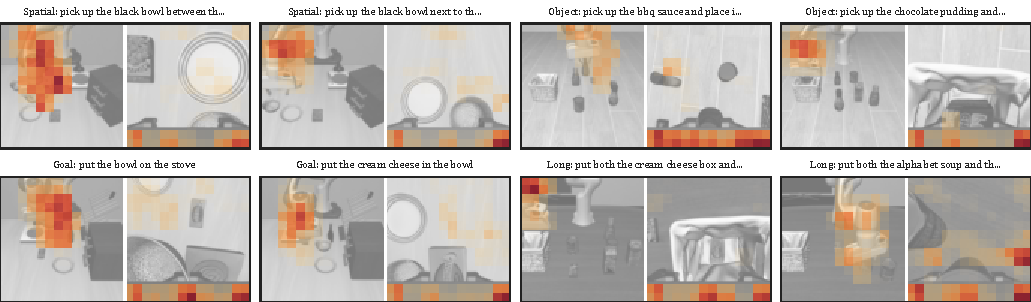
\includegraphics[width=\textwidth]{figures/supp_gaze_maps.pdf}
  \caption{Reader metric of single contexts on Fast-WAM, two from each LIBERO suite.
  Each panel shows the third-person view (left) and the wrist view (right) of the first predicted frame; the color of a token is its share of the trace of the metric estimated on that context alone, normalized within the panel, with the color scale of \cref{fig:obs:gaze}.}
  \label{fig:supp:gaze}
\end{figure*}

\section{Real-world experiments}
\label{sec:supp:real}

\paragraph{Tasks.}
\cref{fig:real} shows one demonstration of each task.
Two-object pick-and-place has three other objects on the table as distractors; this long-horizon task tests whether the quantized model completes a multi-step sequence and picks the named objects.
Shelf placement is a precise insertion under the top board of the shelf that the third-person camera only partly sees, so the final placement relies on the wrist view.
In box stacking, each box must land on the small top face of the one below, which tests placement precision.

\paragraph{Data.}
Each demonstration records a third-person and a wrist RGB camera (Intel RealSense, $320\times240$) and the joint state of the arm at 30\,Hz.
We collect 80 demonstrations for pick-and-place (11.7\,s on average), 75 for shelf placement (7.7\,s) and 80 for box stacking (11.6\,s), with one language instruction per task: ``place the red apple and green cube to the box'', ``place the bowl to the second floor'' and ``pile the boxes''.
We subsample the demonstrations to 10\,Hz, so that a chunk of 32 actions spans 3.2\,s.
Each demonstration is read at the three possible offsets of the subsampling, which gives 705 training sequences that together cover every recorded frame.
The action is the joint target of the next 10\,Hz step, relative to the current joints for the six arm joints and absolute for the gripper; the two views are resized to $224 \times 224$ and placed side by side, as in the LIBERO model.

\paragraph{Fine-tuning.}
We fine-tune one BF16 model on the three tasks jointly, starting from a Fast-WAM LIBERO checkpoint.
Training runs for 6{,}000 steps with a batch size of 32 and a learning rate of $10^{-4}$ with cosine decay, and takes 8.5 hours on four NVIDIA A100 GPUs.
All demonstrations are used for training.

\paragraph{Quantization.}
We apply to the fine-tuned model the pipeline of the simulation experiments, with the same network, rotations, budget and refinement.
The 80 calibration contexts are frames of the demonstrations, 27, 27 and 26 from the three tasks, and the reader metric is re-estimated on them with four probes each; the allocation uses 16 of them.
The metric is as concentrated as in simulation: its effective rank is 27.4, the first predicted frame carries 94\% of its trace, and its diagonal correlates at 0.96 across two halves of the contexts.
The allocation differs from that of the LIBERO model.
It refines 66 of the 98 observation tokens and all 98 entries of the observation cache, and places most of the refined future tokens at the first denoising step (84 of 196), which gives 4.58 bits for the activations and 4.94 bits for the caches.
The allocation thus adapts to the model at hand, with no setting changed by hand.

\paragraph{Trial protocol.}
Every method runs 20 trials per task, two from each of 10 initial placements marked on the table, and the order of the methods is randomized at every placement.
A pick-and-place trial succeeds when both named objects rest inside the box within 60\,s, and its first stage when the apple does.
A shelf trial succeeds when the bowl stands on the second floor of the shelf after the gripper has released it, within 45\,s.
A stacking trial succeeds when both boxes stay stacked for 3\,s after the last release, within 60\,s.
A trial also ends when an object leaves the workspace.

\section{Visualizations}
\label{sec:supp:vis}
\cref{fig:supp:gaze} shows the reader metric of single contexts, estimated from the four probes of each context alone, over the frame that the BF16 model predicts for it.
In the third-person view, the metric follows the arm and the gripper as they move from one scene to the next; in the wrist view, it stays at the lower edge of the image, where the fingers of the gripper are.
The background, the distractor objects and most of the table carry almost none of it.
This is the pattern behind Observation~3: the locations that the reader depends on are few and tied to the robot, so a selection that follows them at run time protects them in every scene.

